\documentclass[10pt]{article}
\usepackage[margin=0.7in]{geometry}
\usepackage{graphicx,mathptmx}
\usepackage[hidelinks]{hyperref}
\title{Finite-size extensions of hashed-factor-base ECDLP}
\author{Source review and proposed implementation directions}
\date{30 October 2026}
\begin{document}
\maketitle
\noindent\textbf{Status.} Planning only: no new implementation, experiment,
theorem, speedup or scalar recovery. The enormous onset belongs to one
general contraction schedule; it is not a lower bound for solving its
particular relation networks. The original manuscript's asymptotic conclusion
is conditional on its cited tensor-contraction claim, not independently
validated here.

\begin{center}
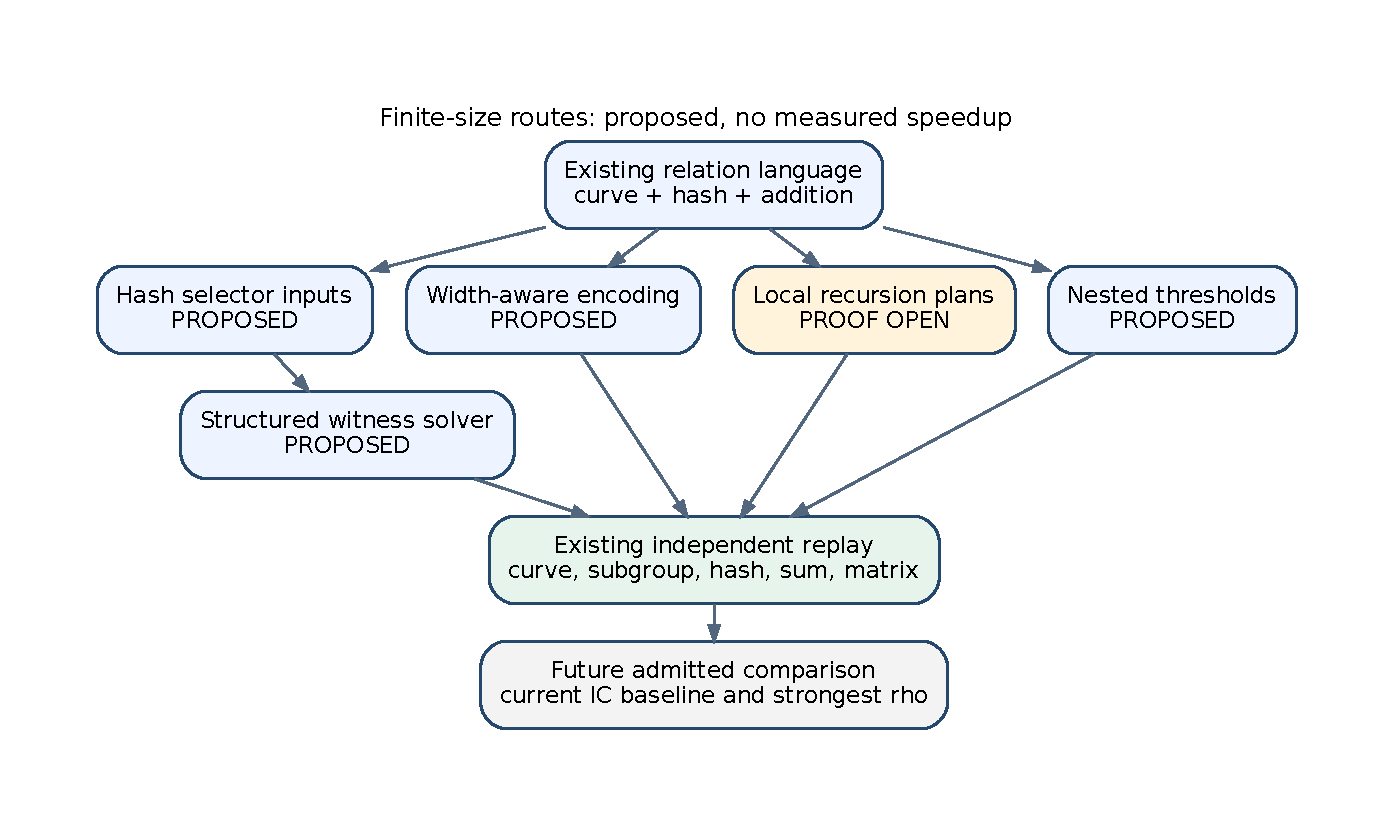
\includegraphics[width=\linewidth,height=3.3in,keepaspectratio]{routes.pdf}
\end{center}

\noindent\textbf{1. Hash selectors as free inputs.}
The native factor-base enumerator already inverts the affine hash on a
bounded threshold interval. Its relation network instead allocates free point
coordinates and constrains membership afterwards. A proposed search should
branch on the interval selector and derive the encoded point. Roughly
$\lceil\log_2\tau\rceil$ free bits per slot replace freely chosen coordinates;
auxiliary arithmetic and decoder work remain. Canonical decoding, invalid-code
rejection and subgroup checks must be faithful. Fixed cofactor projection can
produce multiple source assignments: assignment counts and distinct
decompositions are different quantities. This reuses an existing inverse map;
enumerating all selector tuples is still generic search.

\medskip\noindent\textbf{2. A structured witness backend.}
A relation needs one verified decomposition. Existing native functional
witnesses avoid repeated counts but still branch over declared free inputs.
A witness-only API plus typed arithmetic constraints could support
propagation, incremental target assumptions and exact SAT/SMT, including
native XOR reasoning for binary fields. Opaque predicate closures are not a
CNF exporter. Earlier binary SAT/enumeration encodings already have negative
scaling evidence in the lead atlas. A new backend must identify useful
pruning and price failures, conflicts and propagation; a wrapper alone is
not an algebraic improvement. Timeouts mean UNKNOWN, never UNSAT.

\medskip\noindent\textbf{3. Optimize contraction width and encoding together.}
Linear edge count and quick construction do not imply small intermediate
tensors. Plan low-arity structured factors, elimination orders and cutsets;
compare Fourier and simpler arithmetic gadgets by their complete finite-size
solve cost. TensorOrder supplies a precedent for graph-decomposition-guided
contraction with explicit factorability assumptions. The older binary
bucket/cutset prototype already encountered large widths on tiny fields;
that is a warning, not a measurement of this native Fourier network. Do not
materialize huge truth tables or use approximate contraction to certify an
exact zero count. Sorting interchangeable summands cannot be transplanted to
distinct slot-specific bases without a new argument.

\medskip\noindent\textbf{4. Instance-certified recursion.}
The literal native schedule divides its logarithmic size parameter by
131072, so machine-indexable graphs never get a positive production scale.
Small forced tests check some transformed contractions against direct counts;
they prove neither general small-parameter validity nor speed. Separate
transformation correctness from sufficient asymptotic shrinkage conditions.
A proposed planner must check packing, coefficient/mode coverage, precision
loss, reconstruction, child sizes, resource limits and termination. Try one
layer with a priced exact fallback. Simply changing epsilon does not inherit
the theorem. This route most directly attacks the same recursion's onset,
and retains a substantial proof gap.

\medskip\noindent\textbf{5. Nested hash thresholds and partial relations.}
Use an inner base and a larger outer base under the same hash. Retain
relations with a bounded number of outer points and eliminate them later.
Price outer-base setup, duplicates, storage, elimination and useful matrix
rank. Preserve slot/point identities and coefficients modulo the odd subgroup
order; binary cycle cancellation alone is insufficient. Earlier binary
large-prime collector observations remain unqualified component evidence,
with rho still ahead, and do not establish a gain here. Frobenius or negation
orbits are another possible constant improvement, requiring rebuilt
membership/enumeration/coverage arguments and an equally optimized rho.

\medskip\noindent\textbf{Decision.}
Start with selector-domain witness search, then a width/propagation-aware
backend. Keep checked adaptive recursion as a separate proof-and-planner
track. Improvement over the current index-calculus baseline is useful even
if rho remains ahead. A draft backlog card retains a possible lower-bit
study; its protocol, driver, curves, checker and cost envelope are not ready.
No experiment ran. Earlier S3 checkpoint upload/readback succeeded; native
image/execution readiness remains a distinct prerequisite. The original
frozen A/B panel, both challenge solves and independent audit stay open.

\section*{Identities, evidence and limits}
\noindent Native source: \texttt{edfadbab5ac71471be7fd2971a9e50825307363f}.
ECCp-131 short Weierstrass fixture:
\begin{quote}\small\ttfamily
p=1550031797834347859248576414813139942411\\
a=1399267573763578815877905235971153316710\\
b=1009296542191532464076260367525816293976\\
r=1550031797834347859219047037805205710577\\
cofactor=1\\
s=3102808443644027376164572183694178153449
\end{quote}
\noindent ECC2K-130 is a separate binary problem; its full parameter source is
linked in README.md. Its field degree 131 has no nontrivial intermediate
subfield. Binary XOR/Frobenius ideas do not automatically transfer to the
prime-field fixture. No new curve-panel input or timed run was generated.
All historical measurements here are source reports, not reproduced results.
No comprehensive novelty audit or independent revalidation of those sources
was performed. No new algebraic theorem is claimed.

\medskip\noindent\textbf{Sources checked.}
\href{https://github.com/bochum-crypto/subexponential-ecdl/tree/1ee44e562b1b9a50ea339f3b8f81112b5a24b96f}{Bochum v0.2, sections 2--3 and cutoff footnote};
\href{https://arxiv.org/html/1908.04381v1}{Dudek et al., TensorOrder};
\href{https://pmc.ncbi.nlm.nih.gov/articles/PMC7334981/}{Trimoska et al., SAT-based binary index calculus};
\href{https://github.com/isogeny-labs/crypto-autoresearcher/tree/fc26d24369e56ad20995380475989c40a5e0e84f/knowledge/leads/ecdlp}{pinned lead atlas};
native relation and recursion code; historical binary bucket/cutset prototype.
README.md links individual source and atlas entries, including negative SAT
scaling and generic-oracle cost scopes. No canonical scoreboard, progress,
curve, performance-gain or study result graph receives a new measured value
or curve-transport edge. Editable diagram and PDF accompany this report.
\end{document}
